This section discusses the implementation of the algorithm, the problems encountered and a comparison with the latest Cuckoo version.

\subsection{Implementing the algorithm}

What follows is a short overview of how the algorithm was implemented, the actual code can be found on GitHub\footnote{\url{https://github.com/MartijnB/cuckoo/tree/multi-url}}.

\begin{enumerate}
\item \textbf{Visit} To support the parallel visiting of URLs in one virtual machine, Cuckoo had to be extended. Support for this was added using tabs, but this left us with a problem to detect when a new URL was feeded to a tab (see \ref{99problems}). To solve this problem, every URL in this PoC is now opened in its own window.

\item \textbf{Process} In this step, the API calls were bundled into ten different events before being added to the graph. If no relation was found between an event and a previous event, an edge was created between the event itself and the event which represents the browser context. The HTTP `Referer' header was used to find relations between HTTP events, essentially creating a referer tree\cite{qui}. \todo{Discuss all relations here?}

\item \textbf{Analyse} To implement the analysis phase of the algorithm, a simple analyser was written that detects process spawns below browsing contexts. Appendix A shows pseudo code of the analyser.

\item \textbf{Report} Reporting is done on the commandline but generated graphs of anomalities are saved to the disk in the folder structure of Cuckoo.
\end{enumerate}

\subsubsection{Problems}
\label{99problems}
%\epigraph{I've got 99 problems but Cuckoo ain't one.}{Adriaan}

\textbf{Opening a new URL in the same browser context} was not detectable by the monitored API calls. On top of that, processes were reused when a browsing context was closed and a new one was opened, this made it essentially the same as reusing the browsing context. Internet Explorer also behaves differently when interacting with the automation interface (COM) compared to real user interaction, leaving us without certain registry values that could be used to detect the opening of a new URL. Therefor we decided to use a new Internet Explorer process for each URL which gives us a process ID per browser context.

\textbf{Working with JSON} was extremely slow in Cuckoo. After the virtual machine has done its work, BSON files are transferred to the host machine. These BSON files are then parsed by Cuckoo and analysed after which a JSON file is written. Our \texttt{mass-analyse.py} depended on this JSON, which made it very slow to use. A BSON parser was written to skip the whole JSON step and thus we were able to work earlier on the data, giving us a dramatic speedup.

\subsection{Running the PoC}

Running the proof of concept is as simple as running Cuckoo and running our Python script. Listing \ref{code:run} shows how the PoC is run. As explained in section \ref{sec:setup} the URL list contains the Top 20 most visited websites and some malware websites. Figure \ref{fig:graph} shows the full graph created in the process phase. Notice the red dots in the top left corner of the graph which indicate process spawns and the purple dots which indicate shell command executions. The analyser run in phase 3 succesfully found this anomality and reports it back to the user. A graph of the browsing context in which this anomality occured is also shown to the user, as can be seen in figure \ref{fig:subgraph}.

\begin{lstlisting}[caption={Mass analyser being run},label={code:run}]
$ python cuckoo.py &
$ python utils/mass-analyse.py url_list.txt
Warning: Task with ID 22 is not yet completed; Waiting...
INFO:root:Parse log....
[...]
PID 2876 'iexplore.exe' spawned from parent PID 2860
Visiting: http://google.com/
PID 3656 'iexplore.exe' spawned from parent PID 2860
Visiting: http://malware-site.com/
PID 2108 'iexplore.exe' spawned from parent PID 2860
Visiting: http://google.nl/
PID 3064 'iexplore.exe' spawned from parent PID 2860
Visiting: http://imdb.com/
PID 1012 'iexplore.exe' spawned from parent PID 2860
Visiting: http://facebook.com/
PID 3728 'control.exe' spawned from parent PID 3656
PID 2848 'repfix.exe' spawned from parent PID 3656
PID 1944 'rundll32.exe' spawned from parent PID 3728
PID 3780 'ynuni.exe' spawned from parent PID 2848
[...]
Analyser 'Subprocess_from_tab': The URL 'http://malware-site.com' spawns a process called 'control.exe', 'repfix.exe', 'rundll32.exe' and     'ynuni.exe'.
\end{lstlisting}

\setcounter{savepage}{\arabic{page}}
\stepcounter{savepage}
\pagebreak

\pagenumbering{gobble}
\begin{figure}[h]
    \centering
    \centerline{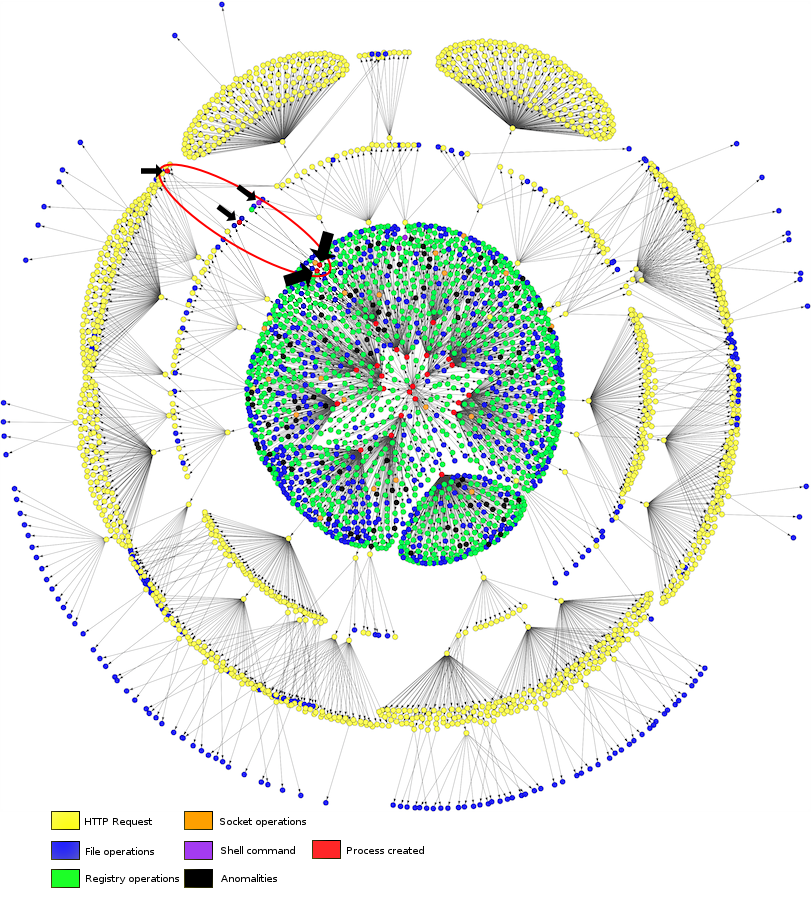
\includegraphics[width=20cm]{Images/graph4.jpg}}
    \caption{An example of the graph generated by visiting the Alexa top 20 and one malicious website. The arrows indicate malicious events generated by the malware.}
    \label{fig:graph}
\end{figure}

\stepcounter{savepage}
\pagebreak

\newgeometry{left=3cm,top=0.1cm,bottom=0.1cm}
\begin{figure}[h]
    \centering
    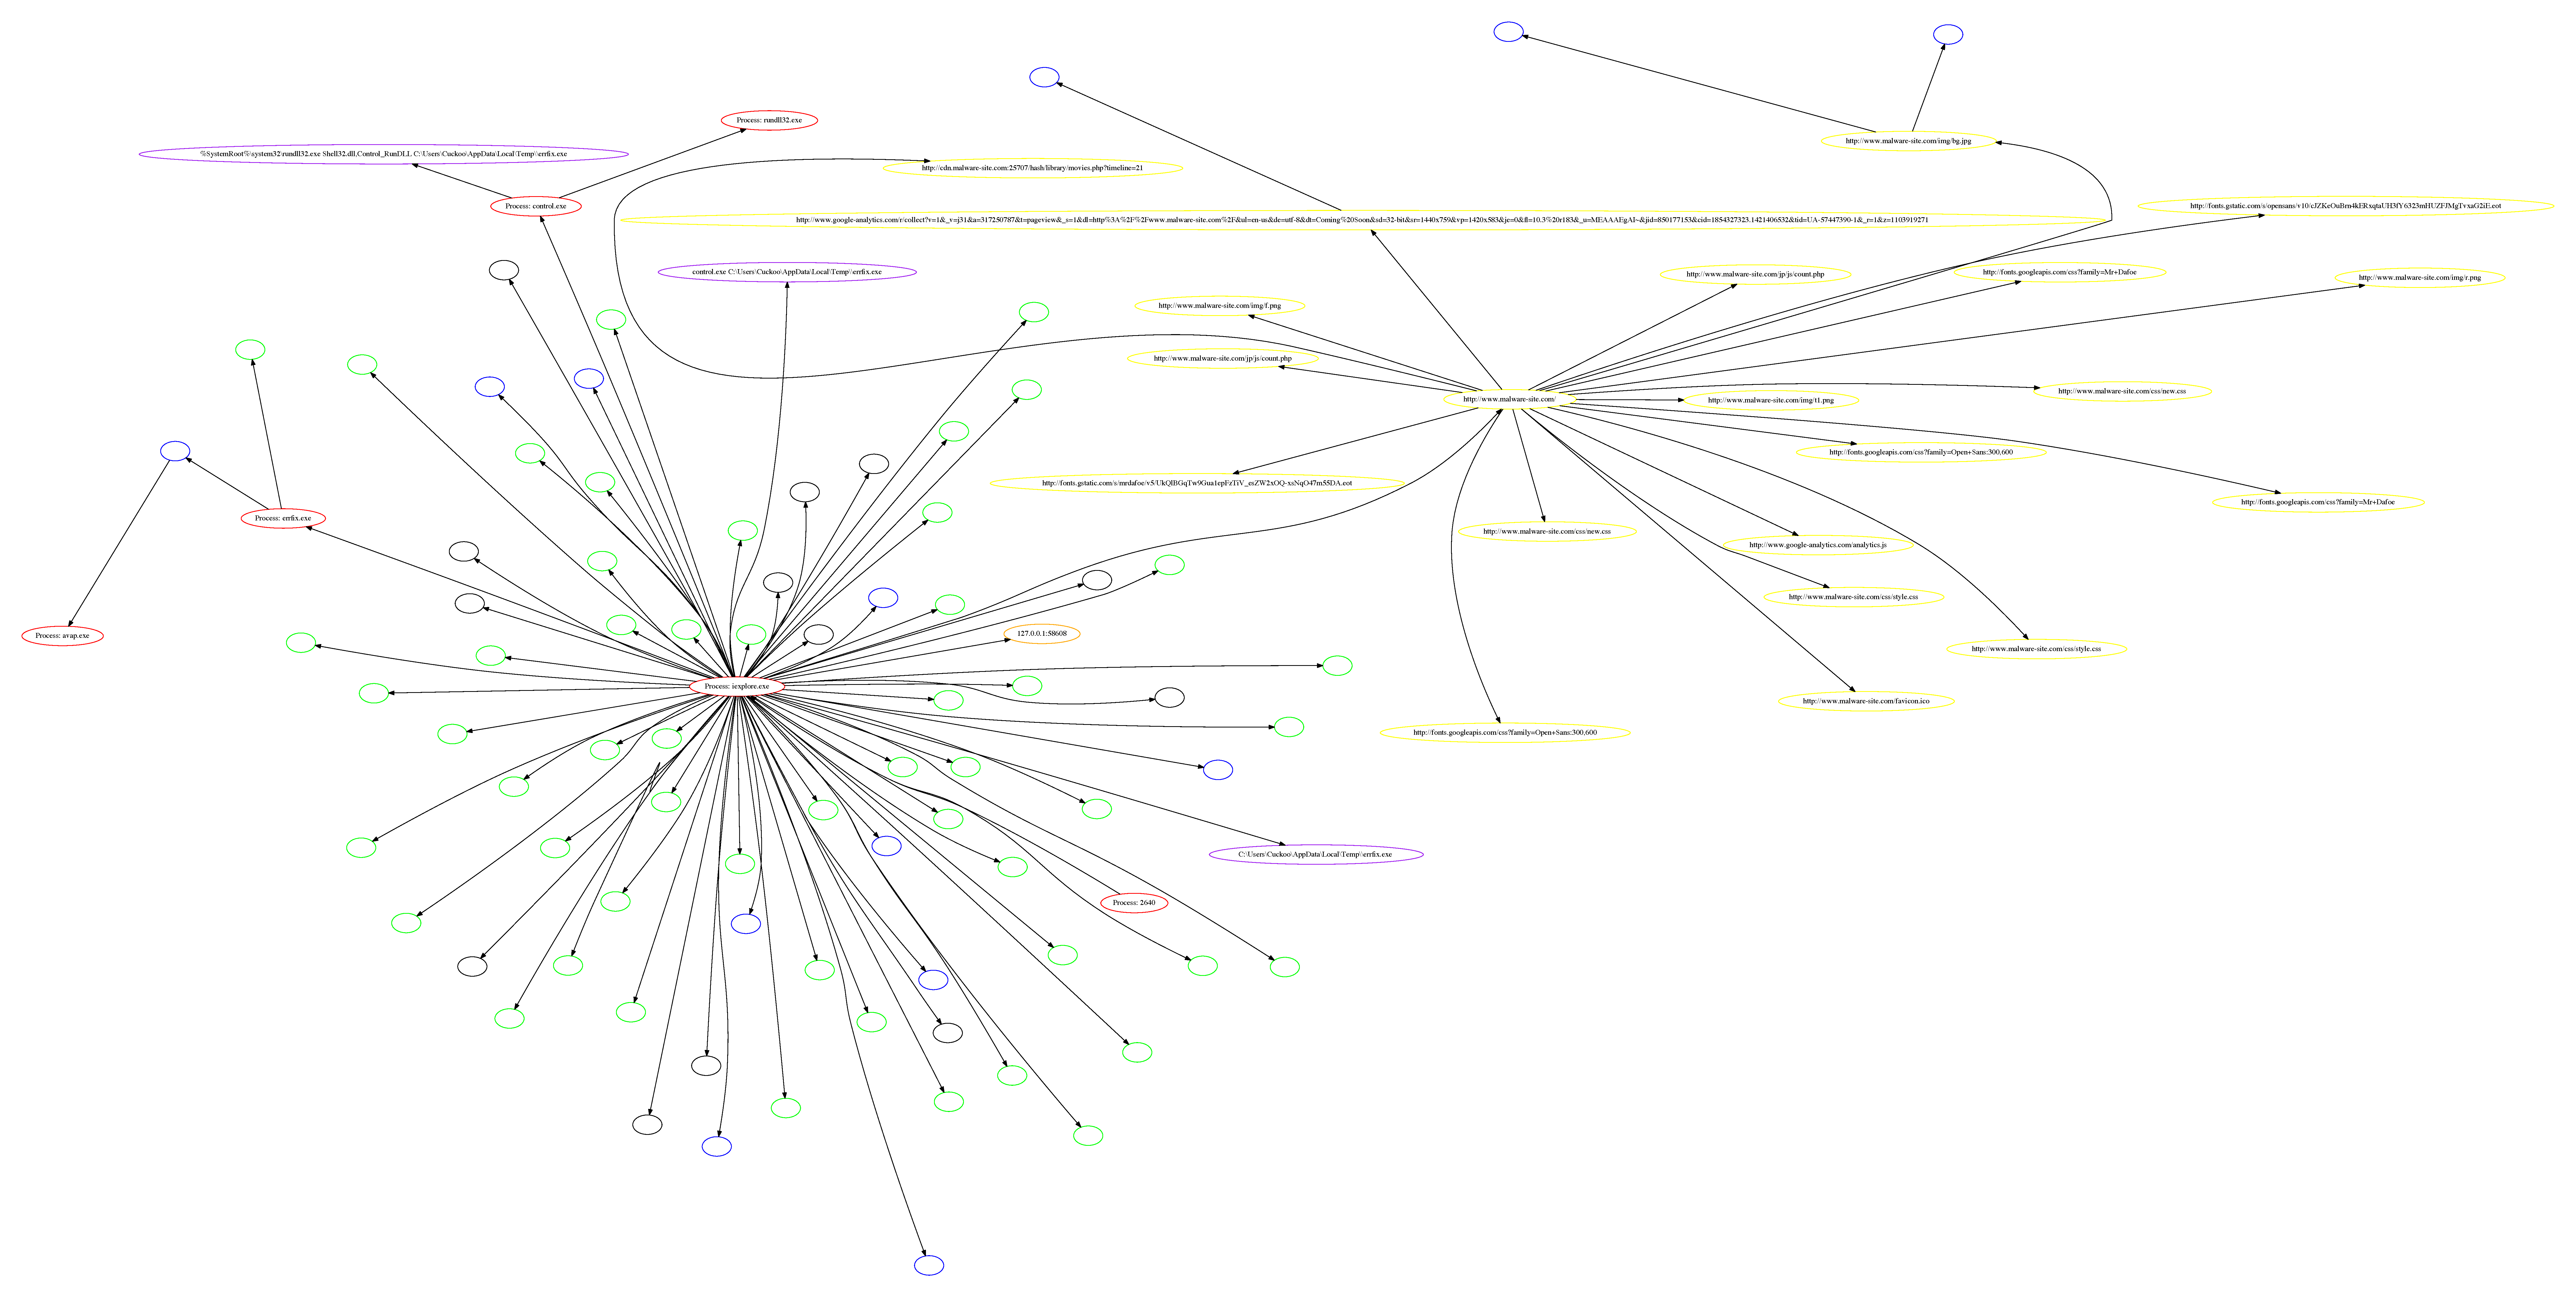
\includegraphics[width=25cm, angle=90]{Images/report_Subprocess_from_tab}
    \caption{An example of the subgraph where a single website was responsible for malware. For clarity, only the labels of visited URLs, involved processes and executed shell commands are shown.}
    \label{fig:subgraph}
\end{figure}

\stepcounter{savepage}
\pagebreak

\restoregeometry
\pagenumbering{arabic}
\setcounter{page}{\thesavepage}

\subsection{Comparison with other malware analysis systems}

To quantify the improvement that was made, several benchmarks were run against our improved version, henceforth called ``Roadrunner''\footnote{http://en.wikipedia.org/wiki/Geococcyx}. Those benchmarks were compared with a development version of Cuckoo 1.2\footnote{\url{https://github.com/cuckoobox/cuckoo/commit/6177071cfd57500fbf1dc17a66f5aff39051c75e}} and Anubis\footnote{\url{http://anubis.iseclab.org/?action=advanced\_form}}, two malware analysis systems which visit URLs sequentially.% The development version of Cuckoo was also used as the base for our development.<-- dit is niet de goeie plaats om dat te zeggen....

The benchmark, for the unmodified Cuckoo, consists of provisioning Cuckoo with one or more URLs until Cuckoo changes the status to ``reported''. Because Roadrunner does not have this status, the benchmark stops when the \texttt{mass-analyse.py} script exits. Anubis reports contain a parameter called ``time needed'' which was used as the benchmark time.

For Roadrunner, benchmarks were executed with 1, 5, 10, 25, 50 and 100 URLs and each benchmark was run 25 times to filter out anomalities. Cuckoo and Anubis were both run 25 times, each with a different URL. Because both only run one URL at a given time, there is no real use in executing it with a different amount of URLs. It will be a linear increase in time with more URLs.

Table \ref{tbl:results} shows the summary\footnote{The raw numbers used to generate the table and graphs can be found in Appendix B.} of the benchmarks. This table gives mean time over 25 runs of Roadrunner with the amount of URLs. For Cuckoo and Anubis, the mean of the 25 runs with 1 URL was calculated and extrapolated to higher URL counts. A comparison in the speed between Cuckoo and Roadrunner has also been made. Although the difference is significant, a sidenote must be made that speed is not the primary goal of Cuckoo and that Cuckoo, if wanted, can be speeded up by configuration tweaks.

Figure \ref{fig:chart-box} and figure \ref{fig:chart-trend} show these numbers in a different way. Figure \ref{fig:chart-box} shows the boxplots of the different runs. We can say that for a lower amount of URLs, there's less variance in the time it takes to complete. Figure \ref{fig:chart-trend} is a visual representation of table \ref{tbl:results}, on the x-axis we see the number of URLs; the y-axis the time it takes to analyse these URLs. 


\begin{figure}[h]
    \centering
    \centerline{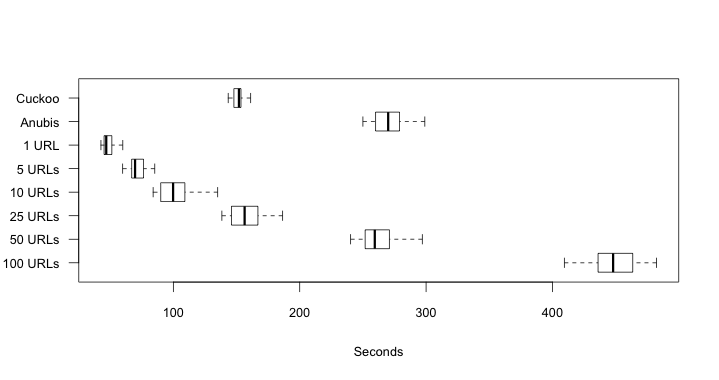
\includegraphics[width=17cm]{Images/chart-box.png}}
    \caption{Less variance on lower URL counts.}
    \label{fig:chart-box}
\end{figure}

\begin{figure}[h]
    \centering
    \centerline{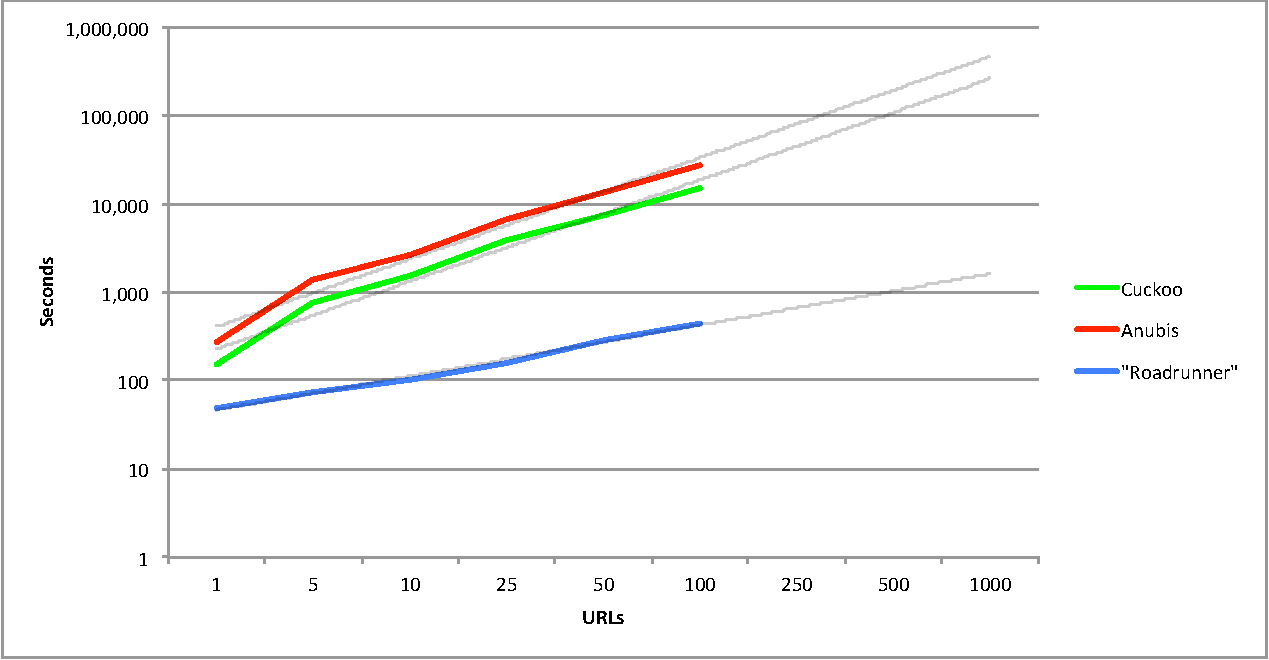
\includegraphics[width=17cm]{Images/chart-trend}}
    \caption{Interpolation and extrapolation of results. Roadrunner is in all cases faster than both systems which run sequentially.}
    \label{fig:chart-trend}
\end{figure}

\begin{table}[h]
\begin{tabular}{@{}lllllll@{}}
\toprule
                                  & 1 URL    & 5 URLs   & 10 URLs      & 25 URLs      & 50 URLs     & 100 URLs \\ \midrule
Anubis       & 273,8s   & 1369,2s   & 2738,4s      & 6846,0s      & 13692,0s     & 27384,0s \\                                  
Cuckoo       & 152,8s   & 764,1s   & 1528,2s      & 3820,5s      & 7640,9s     & 15281,8s \\
Roadrunner& 48,8s    & 74,8s    & 102,4s       & 160,1s       & 286,4s      & 450,9s   \\
Improvement(\%)                   & 313,1\%  & 1021,5\% & 1492,4\%     & 2386,3\%     & 2667,9\%    & 3389,2\% \\ \bottomrule
\end{tabular}
\caption{Mean runtime of Cuckoo, Roadrunner and Anubis. Time in seconds.}
\label{tbl:results}
\end{table}
